% !Mode:: "TeX:UTF-8"

\chapter{系统设计}

\section{App整体设计}
客户端主要是组成页面和处理逻辑的文件,用户在客户端的操作会向服务端发送https请求,服务端收到请求后根据匹配的路由调用函数处理请求,处理结束后向服务端返回响应。
\begin{figure}[h]
	\centering
	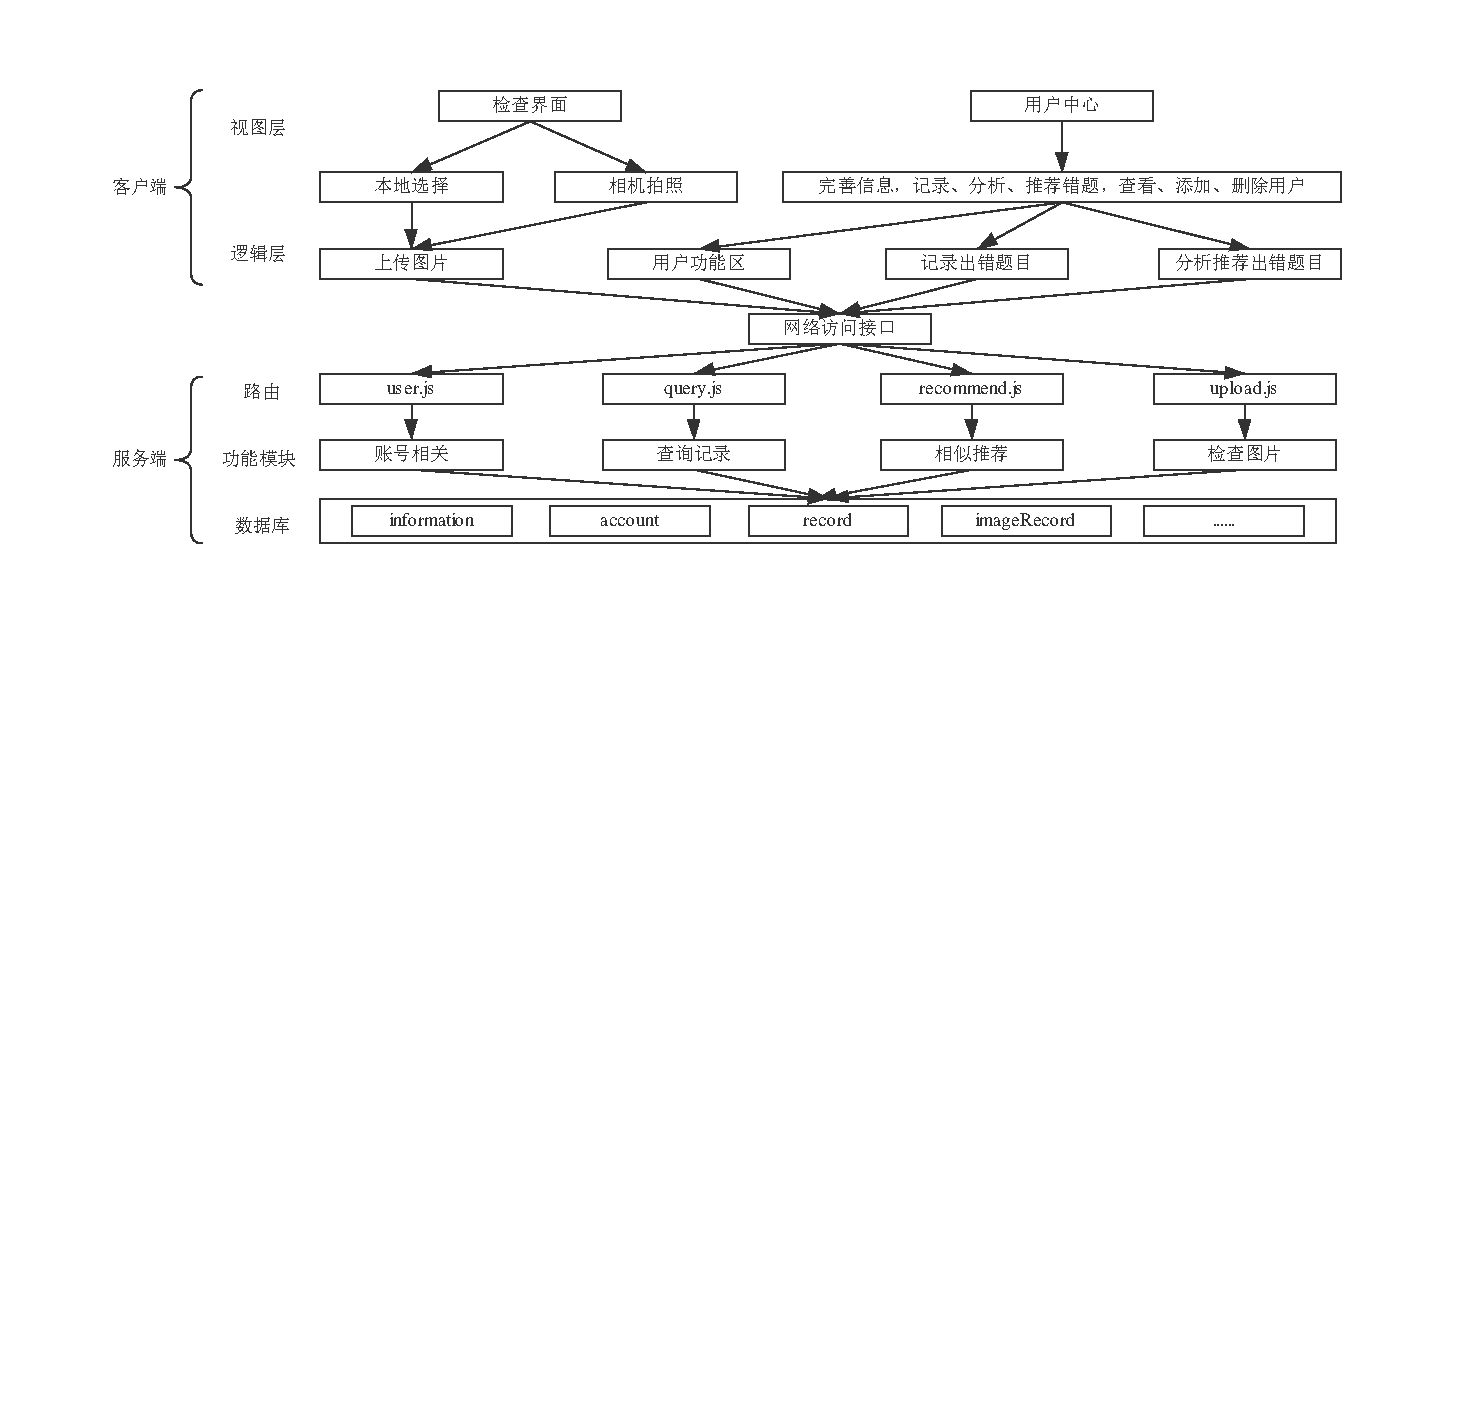
\includegraphics[width=350bp]{picture/overallDesign.pdf}
	\caption{整体设计}
	\label{fig:}
\end{figure}
\par
\section{App客户端设计}
\begin{figure}[h]
	\centering
	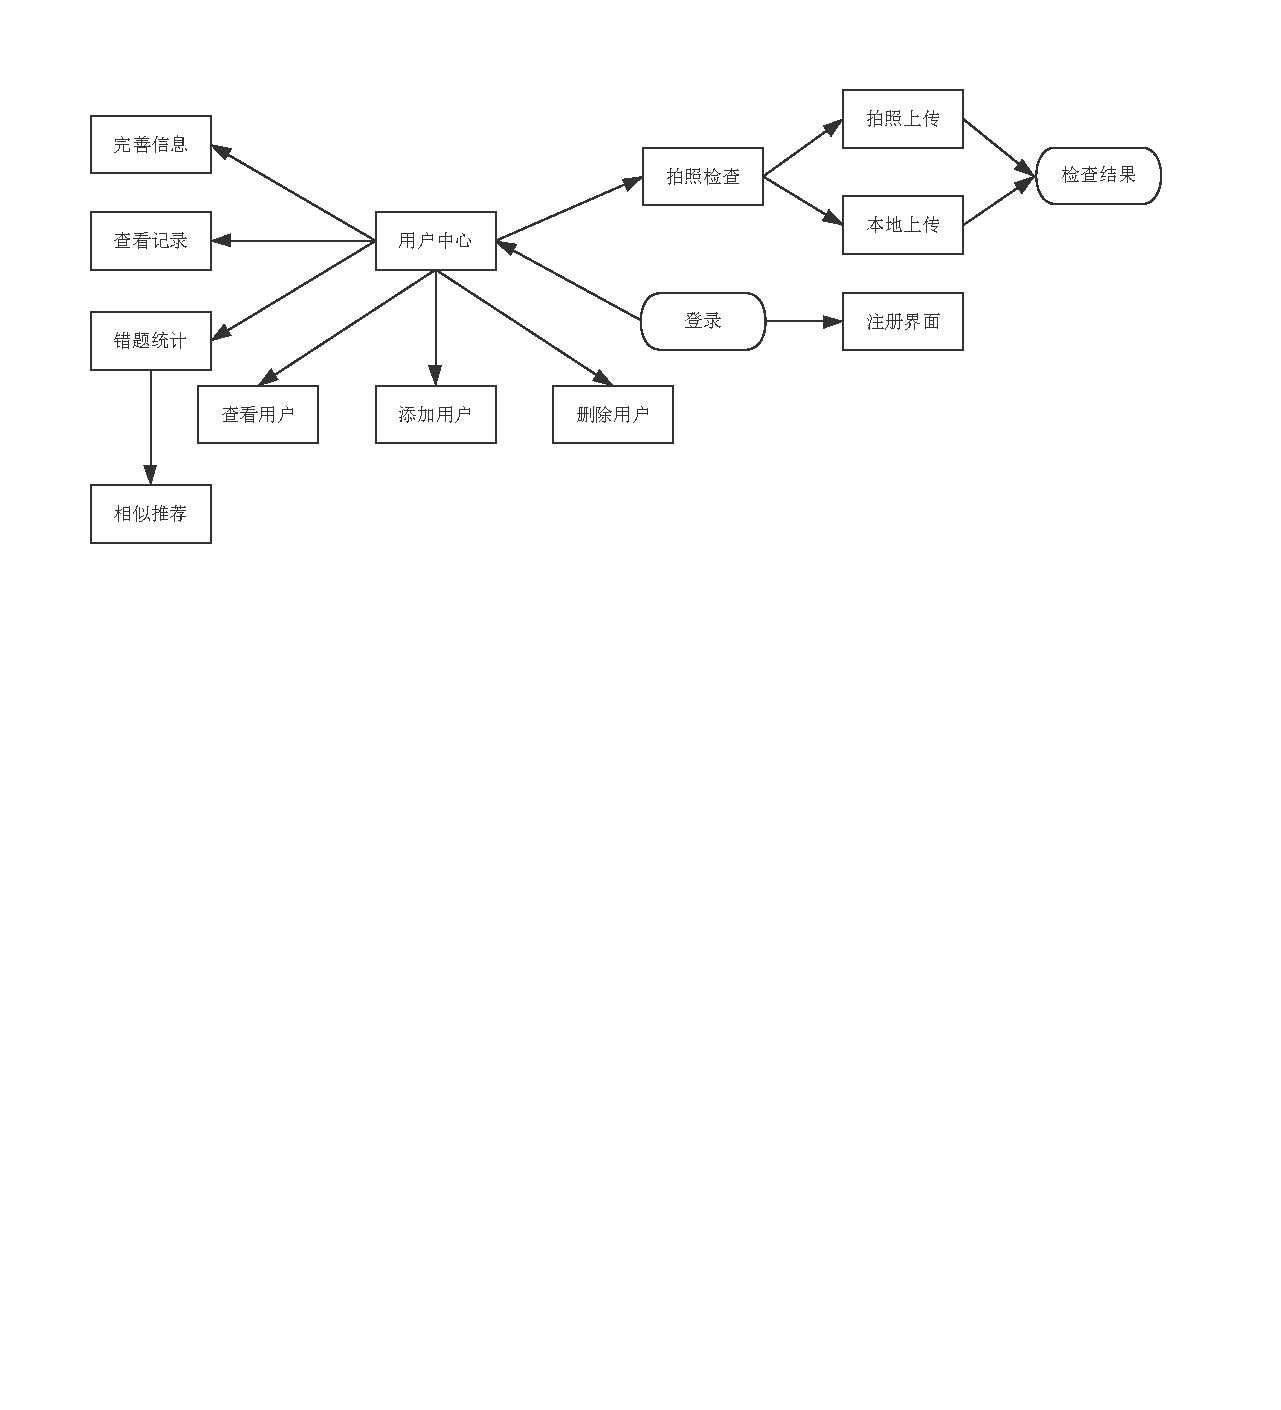
\includegraphics[width=350bp]{picture/page.pdf}
	\caption{客户端页面流程图}
	\label{fig:}
\end{figure}

根据需求实现客户端页面,用户如果未登录,在应用启动后首先会弹出登陆界面,用户登陆后会跳转到用户中心界面,不同角色的用户在用户中心看到的跳转选项是不同的。学生与老师可以使用完善信息、查看历史检查记录和错题统计功能,学生只能看到自己的错题统计,老师可以看到所有学生的错题统计,管理员在用户中心可以使用查看、添加和删除用户的功能。客户端底部有两个导航栏:拍照检查和用户中心。拍照检查提供拍照上传和本地上传两种选择,图片上传结束后会跳转到结果界面。

\section{服务器设计}
服务端使用Express框架实现,服务端程序分为两层,第一层用于接收App端传来的各种数据和请求,本项目针对App功能编写了四个js文件users.js、upload.js、query.js、recommend.js分别用于处理用户账号、图片检查、数据查询和算式推荐请求。第二层根据第一层收到的请求,调用函数处理传来的数据,进行相关的数据库操作。如果是检查图片内容的请求,会调用子进程处理图片,子进程执行用来处理图像的python程序,然后把处理后的结果图片存储在硬盘上,同时把识别出的算式返回给父进程,父进程把这些内容存储到数据库并发送到客户端。

\section{数据库设计}

\begin{figure}[h!]
	\centering
	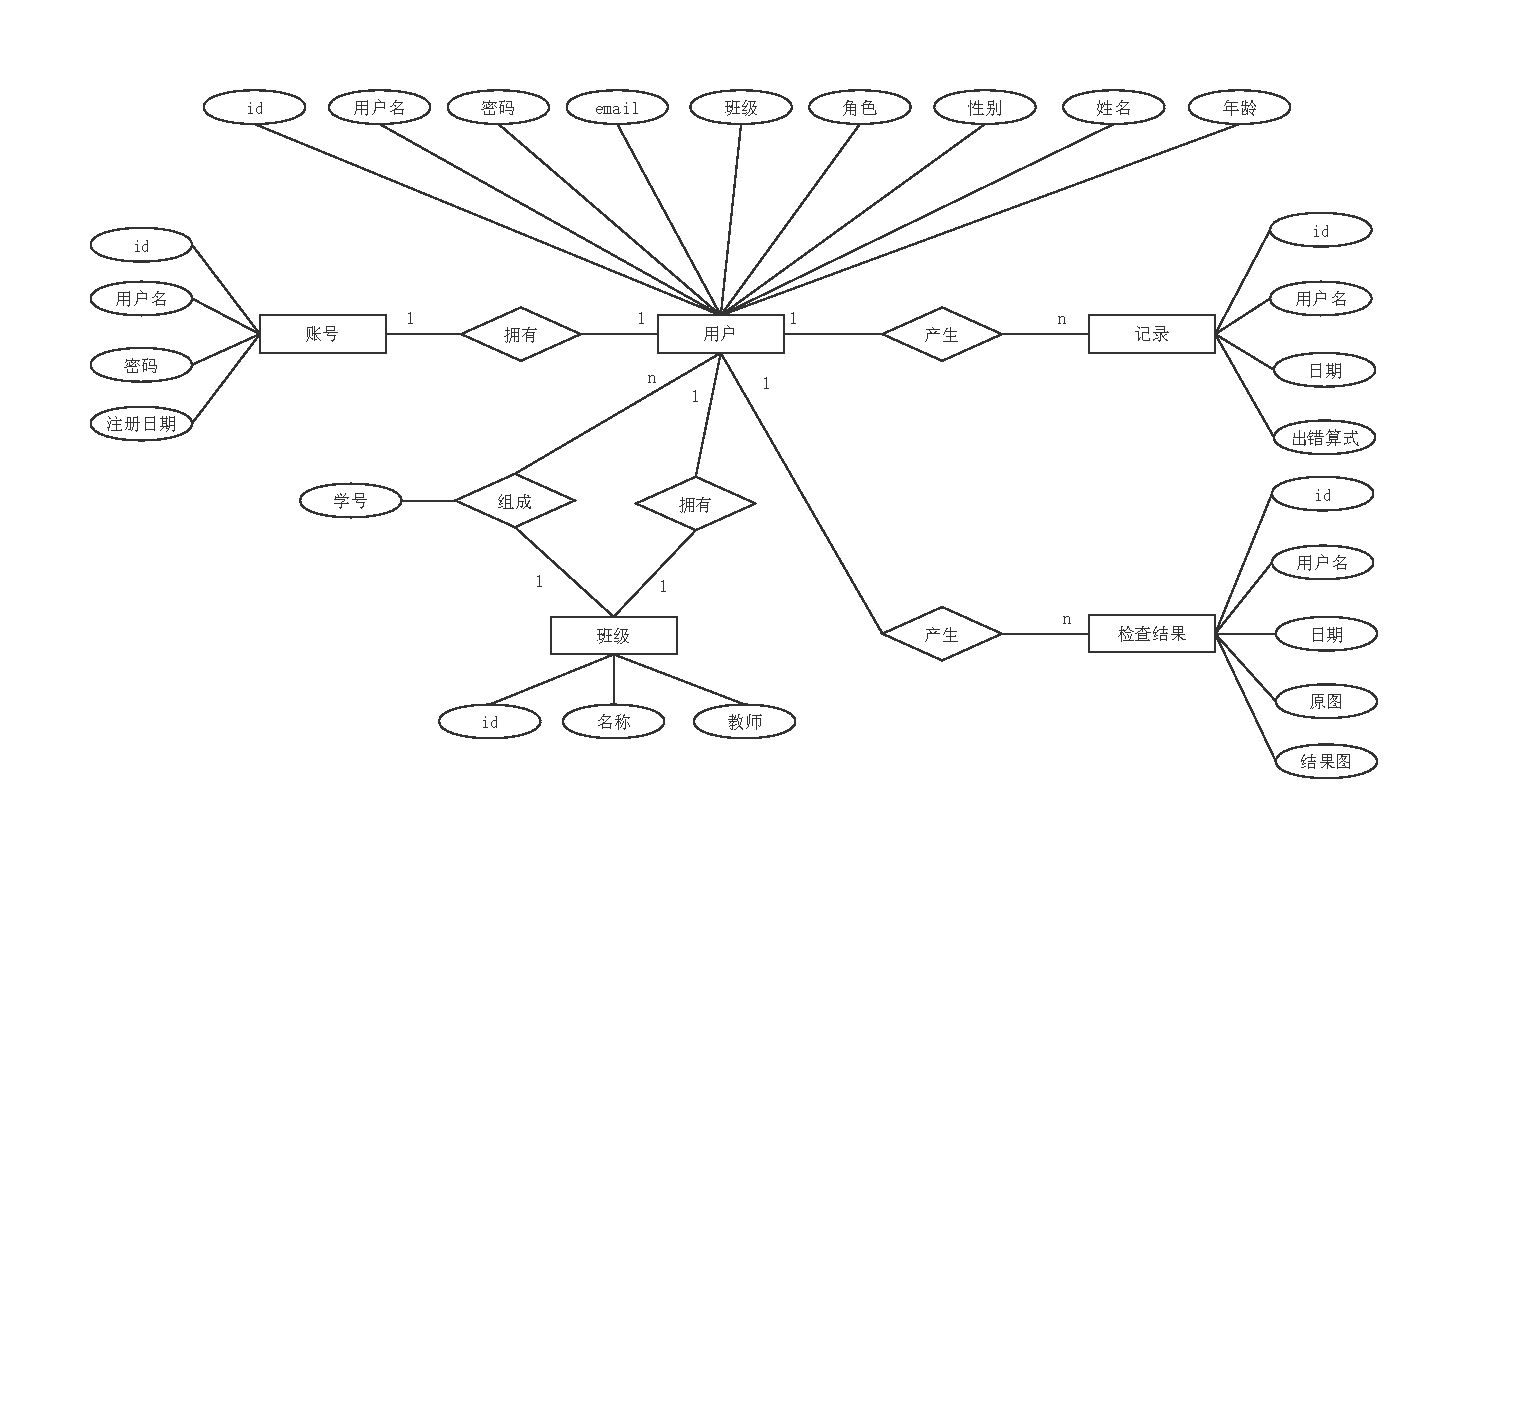
\includegraphics[width=350bp]{picture/E-R.pdf}
	\caption{数据库E-R图}
	\label{fig:}
\end{figure}
\par

\begin{table}[h!]
\begin{center}
\caption{用户信息表}
\begin{tabular}{|c|c|c|c|}
 \hline
 字段名 & 类型 & 代表内容 & 其他\\
 \hline
id & int(11) & id & auto increment, PRI \\
 \hline
name & varchar(45) & 用户名 & PRI \\
 \hline
role & varchar(45) & 电子邮箱地址 & - \\
 \hline
 password & varchar(45) & 角色 & - \\
  \hline
 trueName & varchar(45) & 真实姓名& - \\
  \hline
 gender & varchar(45) & 性别 & - \\
  \hline
  age & varchar(45) & 年龄 & - \\
  \hline
  class & varchar(45) & 班级 & - \\
  \hline
\end{tabular}
\end{center}
\end{table}
\par

\begin{table}[h!]
\begin{center}
\caption{账号表}
\begin{tabular}{|c|c|c|c|}
 \hline
 字段名 & 类型 & 代表内容 & 其他\\
 \hline
id & int(11) & id & auto increment, PRI \\
 \hline
name & varchar(45) & 用户名 & PRI \\
 \hline
password & varchar(45) & 密码 & - \\
  \hline
 date & varchar(45) & 注册日期 & - \\
  \hline
\end{tabular}
\end{center}
\end{table}
\par

\begin{table}[h!]
\begin{center}
\caption{错题记录表}
\begin{tabular}{|c|c|c|c|}
 \hline
 字段名 & 类型 & 代表内容 & 其他\\
 \hline
id & int(11) & id & auto increment, PRI \\
 \hline
name & varchar(45) & 用户名 & PRI \\
 \hline
 date & varchar(45) &  出错日期 & - \\
  \hline
  formula & varchar(45) & 出错算式 & - \\
  \hline
\end{tabular}
\end{center}
\end{table}
\par

\begin{table}[h!]
\begin{center}
\caption{检查结果表}
\begin{tabular}{|c|c|c|c|}
 \hline
 字段名 & 类型 & 代表内容 & 其他\\
 \hline
id & int(11) & id & auto increment, PRI \\
 \hline
name & varchar(45) & 用户名 & PRI \\
 \hline
 date & varchar(45) & 出错日期 & - \\
  \hline
  originalPath & varchar(255) & 原图的路径 & - \\
  \hline
   resultPath & varchar(255) & 结果图片的路径 & - \\
  \hline
\end{tabular}
\end{center}
\end{table}
\par

\begin{table}[h!]
\begin{center}
\caption{班级表}
\begin{tabular}{|c|c|c|c|}
\hline
 字段名 & 类型 & 代表内容 & 其他\\
\hline
id & int(11) & id & auto increment, PRI \\
\hline
name & varchar(45) & 用户名 & PRI \\
\hline
 teacher & varchar(45) & 老师用户名 & - \\
 \hline
\end{tabular}
\end{center}
\end{table}
\newpage

\section{网络访问接口}
客户端与服务端进行数据交换的网络接口\\
https://www.haohybh.cn/users/\\
查询用户是否已经登陆,如果未登陆https响应返回”none”;\\
https://www.haohybh.cn/users/login\\
查询用户名和密码是否匹配,如果匹配返回用户角色;\\
https://www.haohybh.cn/users/addUser\\
添加用户,如果操作成功返回{success: ”yes”},失败返回{success: “no”};\\
https://www.haohybh.cn/users/deleteUser\\
删除用户,如果操作成功返回{success: ”yes”},失败返回{success: “no”};\\
https://www.haohybh.cn/users/queryName\\
查询用户名是否存在,如果已经存在返回{exist: “yes”},不存在返回{exist: “no”};\\
https://www.haohybh.cn/users/queryAllUser\\
查询所有用户的用户名,如果存在用户返回所有用户的用户名,否则返回{exist: “no”};\\
https://www.haohybh.cn/users/addAttributes\\
添加用户信息,如果操作成功返回{success: ”yes”},失败返回{success: “no”};\\
https://www.haohybh.cn/fileUpload\\
提交要检查的图片,处理结束后返回{path: “xxx.jpg”};\\
https://www.haohybh.cn/check\\
查询本用户的错误记录,如果存在相应的记录返回查询结果,否则返回{exist: “no”};\\
https://www.haohybh.cn/check/teacher\\
查询所有用户的错误记录,如果存在相应的记录返回查询结果,否则返回{exist: “no”};\\
https://www.haohybh.cn/check/history\\
查询本用户的历史检查记录,如果存在相应的记录返回查询结果,否则返回{exist: “no”};\\

\section{本章小结}














